\documentclass[11pt,a4paper]{article}
\usepackage[latin1]{inputenc}
\usepackage[spanish]{babel}
\usepackage{amsmath}
\usepackage{amsfonts}
\usepackage{amssymb}
\usepackage{graphicx}
\usepackage[left=2cm,right=2cm,top=2cm,bottom=2cm]{geometry}
\author{Samuel Caleb Mart�nez Hern�ndez}
\title{Par de rotaci�n y cuaternios unitarios}
\begin{document}
\maketitle
\begin{center}
Ingenier�a en mecatr�nica
\end{center}
\begin{center}

\includegraphics[width=7cm]{EV1_3/logo.png} 
\end{center}
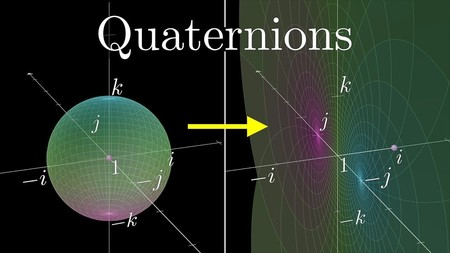
\includegraphics[scale=1]{EV1_3/1.jpg} 
\section{Cuaternio Unitario}
Un cuaternio unitario es un conjunto de 2 datos y es representado por la letra "Q" 
\begin{eqnarray}
Q=(\rceil ,\varepsilon) 
\end{eqnarray}
El primer s�mbolo es el escalar y el segundo es el vectorial.
\begin{center}
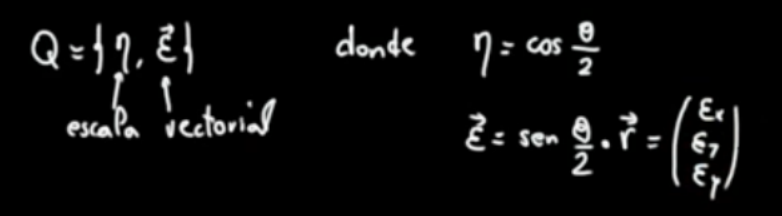
\includegraphics[scale=0.7]{EV1_3/2.png}
\end{center}
 
Estos datos se subdividen en 4, tomando en cuenta el enfasis que se tiene en "x","y" y "z", como parte de euler (vectorial).

\section{Matriz de cambio de orientaci�n a partir del cuaternio} 
\begin{center}
\begin{figure}[hbtp]
\centering
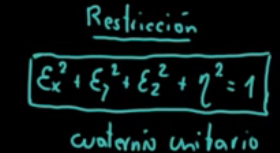
\includegraphics[scale=0.8]{EV1_3/3.png}
\caption{Restricci�n}
\end{figure}

\end{center}
Cuando se utiliza la restricci�n del cuaternio para poder hacer la matriz de cambio que se relaciona con la rotaci�n, ademas de tomar las funciones de la parte escalar y vectorial, nos queda una matriz de este estilo...

\begin{center}
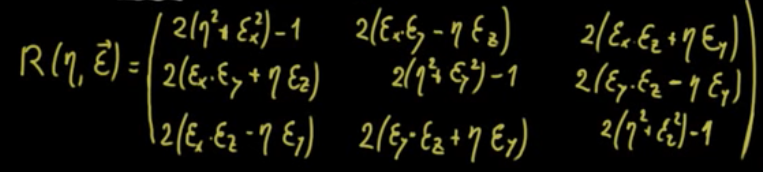
\includegraphics[scale=0.5]{EV1_3/4.png} 
\end{center}

\section{Rotaci�n}
Rotaci�n es el movimiento de cambio de orientaci�n de un cuerpo o un sistema de referencia de forma que una l�nea (llamada eje de rotaci�n)o un punto parece fijo. La rotaci�n de un cuerpo se presenta mediante un operador que afecta un conjunto de puntos o vectores. 

\section{�Que resulta de esto?}
Desde un enfoque practico, cuando se tienen los cuatro valores num�ricos del cuaternio, es decir, la parte escalar y los tres de la parte vectorial, podemos conocer la matriz de cambio de orientaci�n del cuaternio. Resulta una composici�n simple y que a comparaci�n de las matrices de rotaci�n, estas son mas eficaces y desde luego estables  hablando.

\section{Aplicaciones}
Como ingeniero me interesa conocer la utilidad de los conocimientos adquiridos, y a juzgar de que los cuaternarios son �tiles en aplicaciones de gr�ficos por computadora, robotica, navegaci�n y mec�nica orbital de sat�lites, se puede llegar a la conclusi�n de que tales conocimientos tienen una muy justificada raz�n de ser, sobre todo si hablamos de cinem�tica de robots.

De esta manera podemos representar las rotaciones y orientaciones de objetos en las tres dimensiones existentes. 

\begin{center}
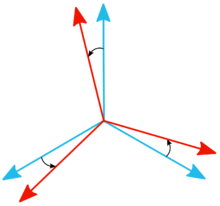
\includegraphics[scale=1]{EV1_3/5.png} 
\end{center}

\paragraph{Referencias}

Del Castillo, G. T. (1999). La representaci�n de rotaciones mediante cuaterniones. Miscelanea Matemtica, 43-50.

\end{document}
